\section{Esercizio 9 -- Processore MIC-1}
\subsection{Analisi dell'architettura}
Il \textbf{MIC-1} è un'architettura microprogrammata che costituisce il livello microarchitetturale di un sistema di elaborazione. Il suo ruolo principale è quello di eseguire le microistruzioni che controllano il funzionamento della CPU a un livello molto dettagliato, traducendo le istruzioni macchina in operazioni elementari.

Importante è il legame tra \textbf{IJVM} (Integer Java Virtual Machine) e \textbf{MIC-1}, fondamentale per comprendere come le istruzioni di un linguaggio macchina vengano effettivamente eseguite dall'hardware attraverso la microprogrammazione.

La sua architettura si basa su un'unità operativa centrale chiamata \textbf{datapath}, che è responsabile dell'elaborazione dei dati e del trasferimento delle informazioni tra i registri e la memoria.

\subsubsection*{Componenti principali del Datapath}

Il datapath del MIC-1 [Figura \ref{fig:mic1_datapath}] è costituito da quattro macro-componenti fondamentali:

\begin{enumerate}
    \item \textbf{Bus di comunicazione con la memoria}: il processore utilizza due bus distinti per comunicare con la memoria principale:
    \begin{itemize}
        \item \textbf{Bus B}: utilizzato per trasferire i dati dai registri interni verso l'ALU e la memoria.
        \item \textbf{Bus C}: utilizzato per scrivere i dati nei registri interni dopo l'elaborazione.
    \end{itemize}

    \item \textbf{ALU (Arithmetic Logic Unit)}: è l'unità aritmetico-logica responsabile dell'esecuzione delle operazioni matematiche e logiche. Può eseguire:
    \begin{itemize}
        \item Operazioni logiche: AND, OR, NOT.
        \item Operazioni aritmetiche: addizione, sottrazione.
        \item Confronti per generare valori di stato (flag).
    \end{itemize}
    L'ALU lavora con due ingressi e fornisce un'uscita che può essere inviata ai registri tramite il bus C.

    \item \textbf{Shifter}: è un'unità che permette di modificare la posizione dei bit nei dati elaborati. Il MIC-1 supporta due tipi di shift:
    \begin{itemize}
        \item \textbf{SLL8 (Shift Left Logical 8)}: sposta i bit di un byte verso sinistra di 8 posizioni, riempiendo con zeri i bit meno significativi. Questa operazione è utile per gestire dati a livello di byte.
        \item \textbf{SRA1 (Shift Right Arithmetic 1)}: sposta i bit verso destra mantenendo il bit più significativo inalterato. Questa operazione viene spesso usata per divisioni o per gestire numeri con segno.
    \end{itemize}

    \item \textbf{Registri interni}: il MIC-1 dispone di \textbf{dieci registri da 8 o 32 bit}, che vengono utilizzati per la gestione della memoria, dello stack e dell'esecuzione delle istruzioni.
    \begin{itemize}
        \item \textbf{Nove registri possono inviare dati sul bus B} (tutti eccetto MAR).
        \item \textbf{Nove registri possono essere caricati dal bus C} (tutti eccetto MBR).
    \end{itemize}
\end{enumerate}

\subsubsection*{Descrizione dei Registri del MIC-1}

\begin{enumerate}
    \item \textbf{Registri per la gestione della memoria}:
    \begin{itemize}
        \item \textbf{CPP (Current Procedure Pointer)}: contiene il puntatore alla procedura corrente, utile per il controllo di flusso nei linguaggi di alto livello.
        \item \textbf{LV (Local Variable Pointer)}: indica l'inizio dello spazio di memoria riservato alle variabili locali di una procedura.
    \end{itemize}

    \item \textbf{Registri per il controllo dell'esecuzione}
    \begin{itemize}
        \item \textbf{PC (Program Counter)}: memorizza l'indirizzo della prossima istruzione da eseguire. Dopo ogni fetch, il valore del PC viene aggiornato per puntare all'istruzione successiva.
    \end{itemize}

    \item \textbf{Registri per l'accesso alla memoria}
    \begin{itemize}
        \item \textbf{MAR (Memory Address Register)}: contiene l'indirizzo della word di memoria da leggere o scrivere. Questo registro non può essere scritto tramite il bus C, ma solo tramite microprogrammazione.
        \item \textbf{MDR (Memory Data Register)}: memorizza la word letta dalla memoria o da scrivere in memoria. È un registro di transito tra il processore e la memoria principale.
    \end{itemize}

    \item \textbf{Registri per la gestione dello stack}
    \begin{itemize}
        \item \textbf{TOS (Top of Stack)}: contiene il valore dell'elemento in cima allo stack, facilitando operazioni rapide senza bisogno di accessi multipli alla memoria.
        \item \textbf{SP (Stack Pointer)}: contiene l'indirizzo dell'elemento in cima allo stack, permettendo di gestire la crescita e la riduzione dello stack in modo efficiente.
    \end{itemize}

    \item \textbf{Registri di supporto per l'esecuzione delle istruzioni}
    \begin{itemize}
        \item \textbf{OPC (Opcode Register)}: registro temporaneo utilizzato per memorizzare il codice operativo di un'istruzione in esecuzione.
        \item \textbf{MBR (Memory Byte Register)}: contiene i byte delle istruzioni mentre vengono decodificate ed eseguite. Questo registro non può essere scritto dal bus C, ma solo letto.
    \end{itemize}

    \item \textbf{Registro speciale per l'ALU}
    \begin{itemize}
        \item \textbf{H (Hosting Register)}: contiene temporaneamente uno degli operandi utilizzati dalla ALU durante l'esecuzione delle operazioni aritmetiche o logiche.
    \end{itemize}
\end{enumerate}

\begin{figure}[h]
    \centering
    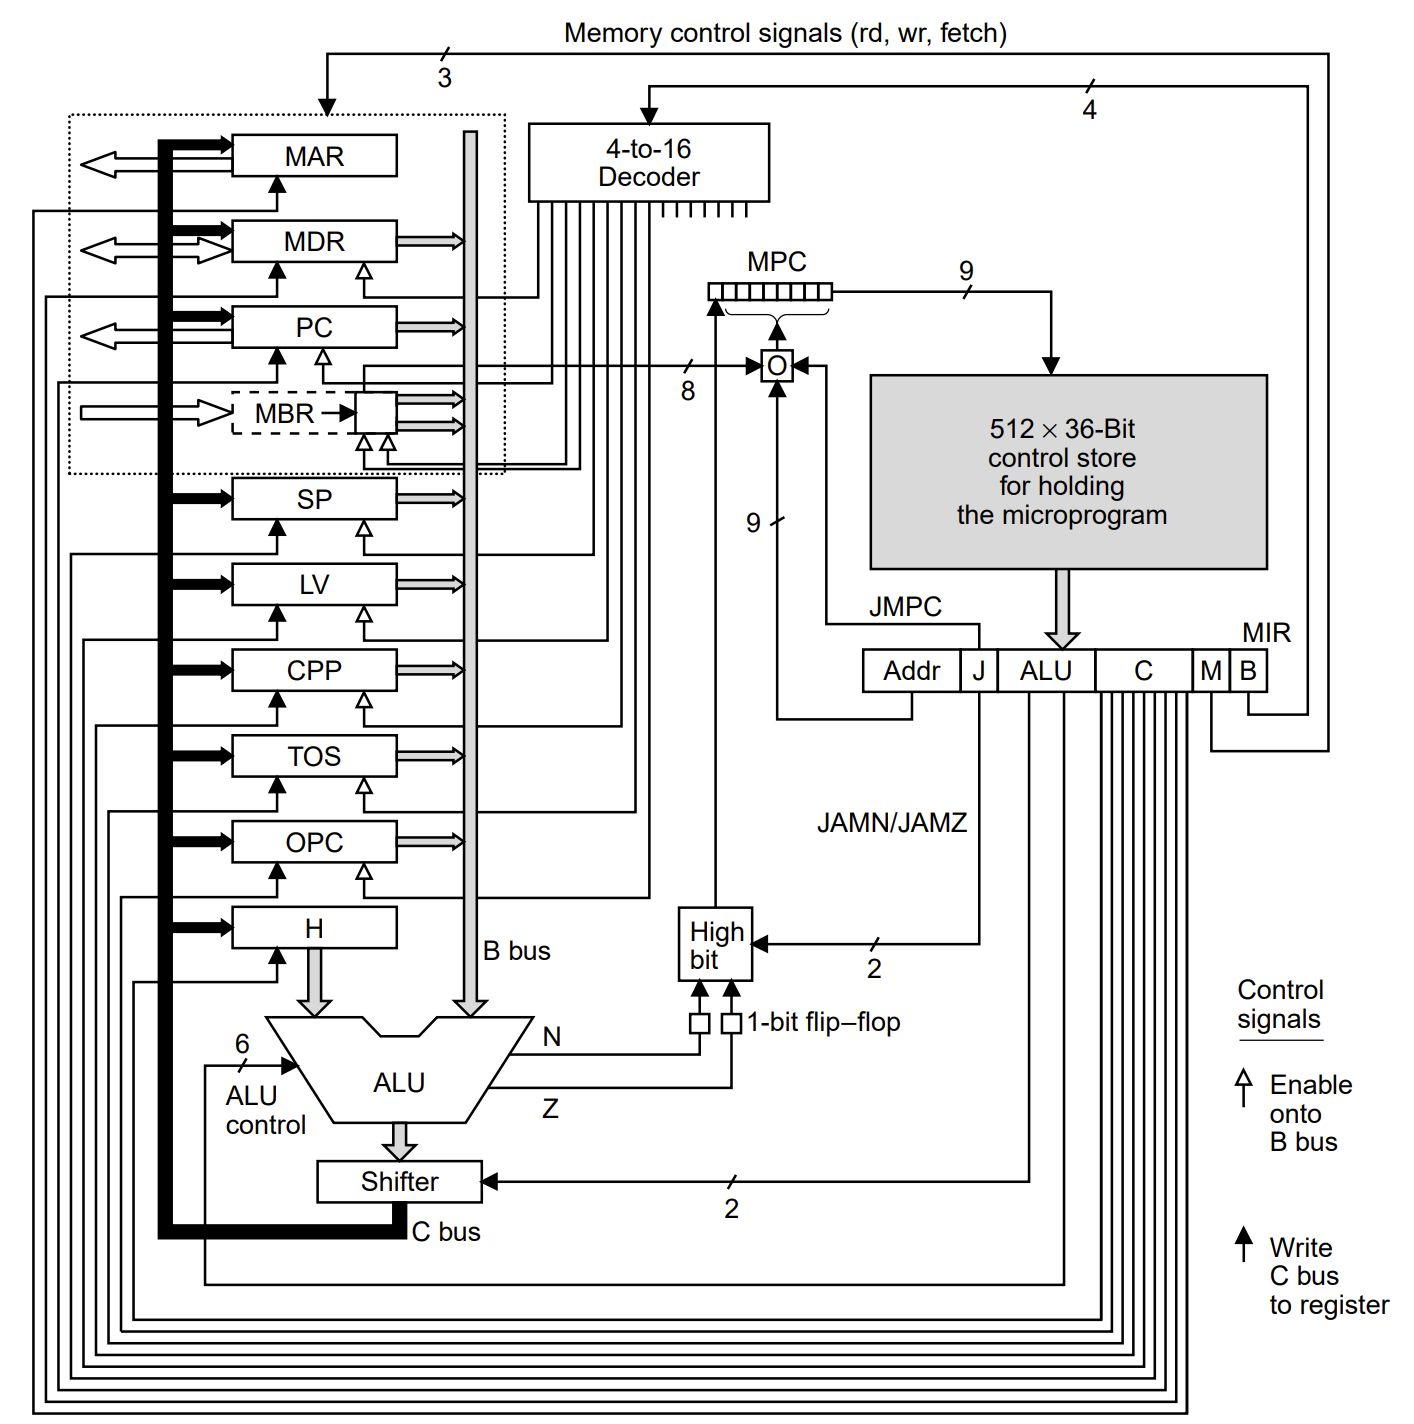
\includegraphics[width=0.8\linewidth]{img/mic1_datapath.jpg}
    \caption{Schema del datapath del processore MIC-1}
    \label{fig:mic1_datapath}
\end{figure}

La comunicazione tra i registri avviene principalmente attraverso il \textbf{bus B}, che fornisce il secondo operando all'ALU. La maggior parte dei registri può inviare il proprio contenuto a questo bus, ma solo uno alla volta può essere abilitato a scrivere su di esso. Al contrario, più registri possono leggere contemporaneamente dal \textbf{bus C}, che rappresenta l'uscita dell'ALU.

I registri utilizzati per la comunicazione con la memoria, che ha una capacità di \textbf{4 GB}, sono:
\begin{itemize}
    \item \textbf{MAR (Memory Address Register)}: contiene l'indirizzo della word da leggere o scrivere.
    \item \textbf{MDR (Memory Data Register)}: immagazzina i dati trasferiti da e verso la memoria.
    \item \textbf{PC (Program Counter)}: mantiene l'indirizzo della prossima istruzione da eseguire.
    \item \textbf{MBR (Memory Byte Register)}: memorizza i byte delle istruzioni man mano che vengono interpretate.
\end{itemize}

Questa architettura utilizza due interfacce di comunicazione con la memoria:
\begin{enumerate}
    \item \textbf{Interfaccia a 32 bit (word-addressable)}: consente sia la lettura che la scrittura ed è gestita dalla coppia \textbf{MAR/MDR}. Il registro \textbf{MDR} può infatti inviare e ricevere dati dalla memoria.
    \item \textbf{Interfaccia a 8 bit (byte-addressable)}: utilizzata esclusivamente per la lettura ed è gestita dal \textbf{PC}, che preleva un byte dagli 8 bit meno significativi dell'\textbf{MBR}. Questa interfaccia può solo leggere dati, poiché l'MBR ha solo una freccia entrante: le istruzioni possono essere solo caricate dalla memoria, non scritte in essa.
\end{enumerate}

È importante sottolineare che:
\begin{itemize}
    \item La coppia \textbf{MAR/MDR} è utilizzata per l'accesso ai dati.
    \item La coppia \textbf{PC/MBR} è impiegata per il recupero e l'esecuzione delle istruzioni del programma.
\end{itemize}

\subsubsection*{Indirizzamento della memoria}

La memoria del processore è organizzata in parole da 8 bit, identificate da un indirizzo a 32 bit, permettendo così di indirizzare $2^{32}$ parole. Tuttavia, l'indirizzamento della memoria varia a seconda che venga utilizzato il \textbf{PC} o il \textbf{MAR}:
\begin{itemize}
    \item Se un indirizzo di byte viene caricato nel \textbf{PC}, il byte corrispondente sarà disponibile nell'\textbf{MBR} al successivo ciclo di clock.
    \item Se l'indirizzo viene caricato nel \textbf{MAR}, al ciclo di clock successivo l'\textbf{MDR} conterrà i 4 byte della word corrispondente.
\end{itemize}

Ciò è possibile perché il \textbf{MAR} esegue uno shift automatico, inserendo "00" nei due bit meno significativi, equivalente a una moltiplicazione per 4. Questo meccanismo permette di convertire l'indirizzo di un byte nell'indirizzo della word corrispondente.

Grazie a questa organizzazione della memoria:
\begin{itemize}
    \item Il recupero dei dati (a 32 bit) richiede un solo accesso in memoria.
    \item Il recupero delle istruzioni (che possono avere lunghezza variabile in multipli del byte) può richiedere più accessi in memoria.
\end{itemize}

\subsubsection*{ALU (Arithmetic Logic Unit)}

Dispone di sei linee di controllo in ingresso e di due segnali in uscita (\textbf{N} e \textbf{Z}), che indicano rispettivamente se il risultato di un'operazione è negativo o nullo. Quando l'ALU deve elaborare due operandi:
\begin{itemize}
    \item Il \textbf{primo operando} viene prelevato da un registro, caricato sul bus B e trasferito all'ALU con una configurazione di controllo che lo pone in uscita su B; successivamente, il valore risultante viene copiato dal bus C nel registro H.
    \item Il \textbf{secondo operando} viene connesso direttamente al bus B.
\end{itemize}

\subsubsection*{Segnali di controllo del datapath}

Il controllo del datapath richiede 29 segnali di controllo, suddivisi in 5 gruppi funzionali:
\begin{enumerate}
    \item \textbf{9 segnali} per controllare la scrittura dal bus C nei registri.
    \item \textbf{9 segnali} per controllare l'abilitazione dei registri verso il bus \textbf{B}, che fornisce l'ingresso destro dell'ALU.
    \item \textbf{8 segnali} per il controllo dell'ALU e dello shifter.
    \item \textbf{2 segnali} per il controllo della lettura/scrittura dei registri MAR e MDR.
    \item \textbf{1 segnale} per il prelievo dalla memoria utilizzando PC/MBR.
\end{enumerate}

Questi segnali determinano le operazioni da eseguire in un singolo ciclo del datapath, che include:
\begin{enumerate}
    \item Il trasferimento di un valore da un registro al bus B.
    \item La propagazione attraverso l'ALU e lo shifter.
    \item Il posizionamento del risultato sul bus C.
    \item La scrittura nei registri appropriati.
\end{enumerate}

Se il segnale di \textbf{memory read data} (per indicare quando deve avvenire una lettura dalla memoria) è attivo, l'operazione in memoria ha inizio alla fine del ciclo del datapath, dopo il caricamento del MAR. Tuttavia, i dati saranno disponibili solo alla fine del ciclo successivo in MBR o MDR e potranno essere utilizzati solo nel ciclo successivo. Poiché MBR e MDR vengono aggiornati sul fronte di salita del clock, possono essere letti anche mentre è in corso una nuova operazione di lettura in memoria. Nonostante ciò, non si verificano ambiguità, poiché i vecchi valori restano utilizzabili fino al caricamento dei nuovi valori nel ciclo successivo.

Per controllare il datapath, sono sufficienti 24 bit di controllo (9 + 4 + 8 + 2 + 1), poiché solo un registro alla volta può scrivere sul bus B.

\subsubsection*{Unità di controllo microprogrammata del MIC-1}

L'unità di controllo del processore \textbf{MIC-1} è microprogrammata e include:
\begin{itemize}
    \item Un generatore degli indirizzi di partenza, che determina l'indirizzo della micro-ROM a cui accedere per eseguire un'operazione.
    \item La memoria di controllo (control store), ovvero la micro-ROM, che contiene le microistruzioni.
    \item Un Program Counter della micro-ROM (MPC), che tiene traccia della microistruzione corrente.
\end{itemize}

La control store è una memoria composta da 512 word, ognuna delle quali è una microistruzione di 36 bit, che contiene l'intero microprogramma del MIC-1.

Le istruzioni ISA rappresentano l'interfaccia con il programmatore. A ciascuna di esse corrisponde una microprocedura, formata da un insieme di microistruzioni memorizzate nella micromemoria. Poiché diverse istruzioni condividono sequenze di esecuzione simili, la memoria è organizzata in modo da evitare la duplicazione delle microistruzioni comuni.

Per ottimizzare questa gestione, il MIC-1 adotta una tecnica in cui ogni microistruzione contiene un campo \textbf{next\_address}, che indica la posizione della successiva microistruzione da eseguire.

I segnali di controllo, che guidano le operazioni della CPU, vengono generati tramite decoder, rendendo l'unità di controllo microprogrammata verticale. In particolare, il MIC-1 utilizza 29 segnali di controllo per il datapath, prodotti direttamente dall'unità di controllo.

Questi segnali determinano il percorso dei dati in un singolo ciclo di clock, mentre un'ulteriore parte della microistruzione stabilisce cosa dovrà avvenire nel ciclo successivo, grazie ai campi Addr e JAM. In generale, la struttura della control word è quella in [Figura \ref{fig:mic1_microinstruction}].

\begin{figure}[h]
    \centering
    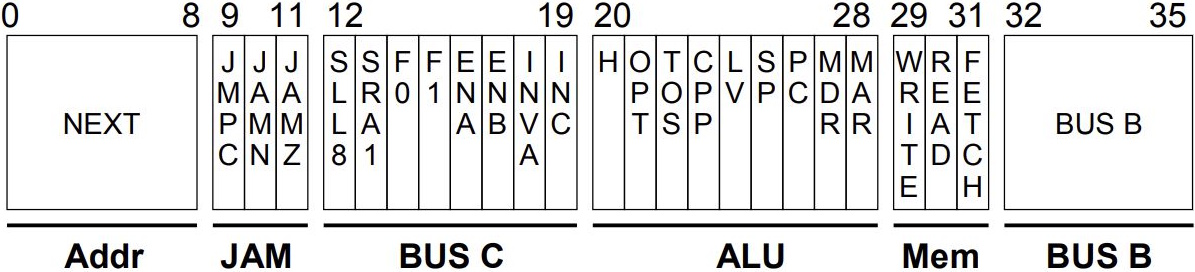
\includegraphics[width=0.6\linewidth]{img/mic1_microinstruction.jpg}
    \caption{Struttura di una microistruzione del MIC-1}
    \label{fig:mic1_microinstruction}
\end{figure}

Il formato di una \textbf{microistruzione} nel processore MIC-1 è suddiviso in 6 campi, ciascuno con una funzione specifica:
\begin{itemize}
    \item \textbf{Campo Addr (9 bit)}: determina l'indirizzo della microistruzione successiva da eseguire (\textbf{next\_address}).
    \item \textbf{Campo JAM (3 bit)}: gestisce le operazioni di salto condizionato, modificando l'indirizzo della prossima microistruzione in base a particolari condizioni.
    \item \textbf{Campo ALU (8 bit)}: specifica le operazioni da eseguire tramite l'ALU e lo shift register.
    \item \textbf{Campo C (9 bit)}: controlla la destinazione dei dati elaborati, determinando su quale registro scrivere.
    \item \textbf{Campo M (3 bit)}: definisce le operazioni di lettura e scrittura della memoria.
    \item \textbf{Campo B (4 bit)}: seleziona la sorgente del bus B, attraverso una codifica compatta.
\end{itemize}

Il formato della microistruzione utilizza 36 bit in totale invece di 41, grazie a un'ottimizzazione nella codifica del campo B [Figura \ref{fig:mic1_microinstruction_format}]. In particolare:
\begin{itemize}
    \item Il segnale di controllo per il bus B è rappresentato su 4 bit anziché 9, mediante una codifica compatta.
    \item Questa scelta richiede l'uso di un decoder, che converte i 4 bit in un segnale completo di 9 bit per il bus B.
    \item Il vantaggio di questa soluzione è una riduzione del numero di fili di controllo che devono attraversare l'intera memoria, limitandoli solo alla parte finale del percorso, ottimizzando così l'hardware.
\end{itemize}

\begin{figure}[h]
    \centering
    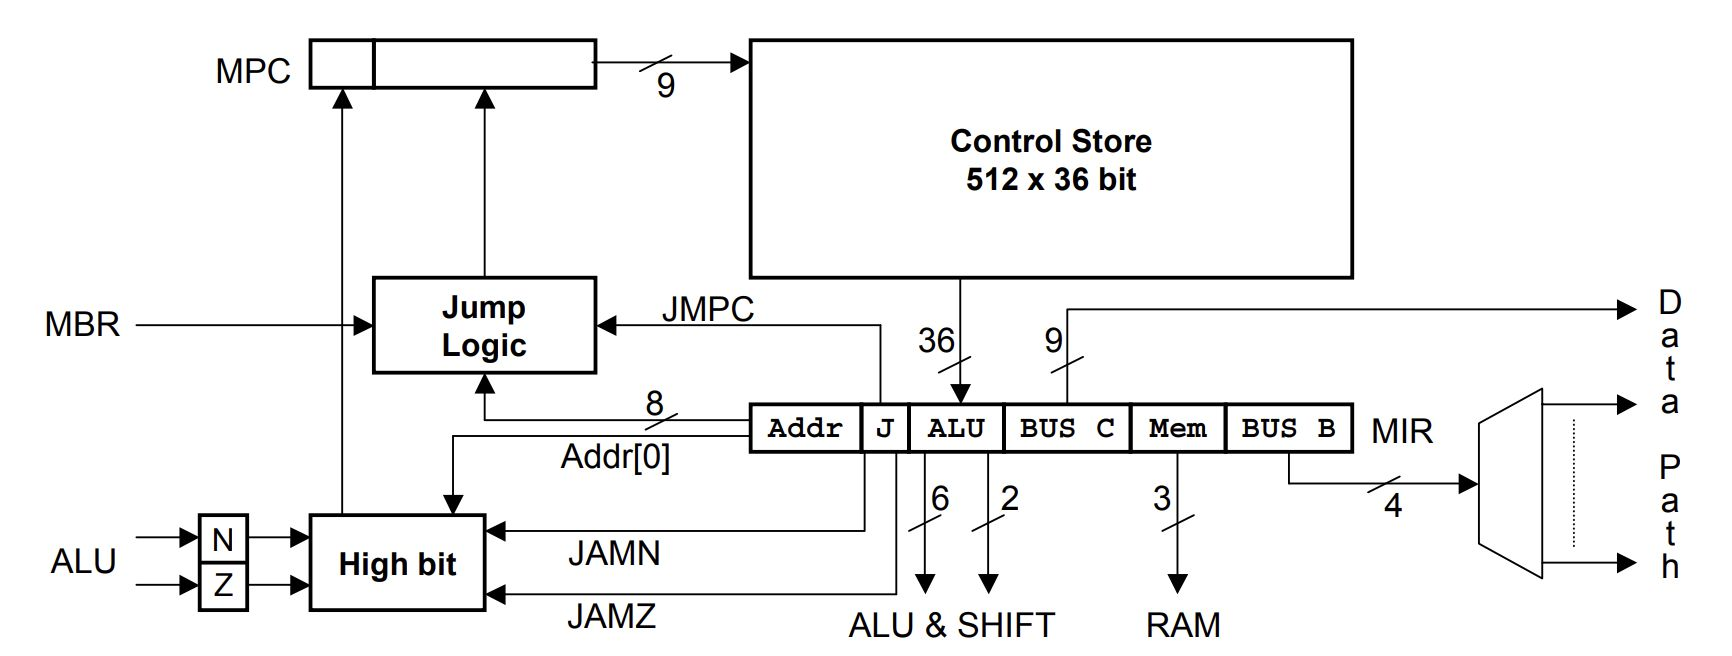
\includegraphics[width=0.8\linewidth]{img/mic1_microinstruction_format.jpg}
    \caption{Formato di una microistruzione del MIC-1}
    \label{fig:mic1_microinstruction_format}
\end{figure}

Il sistema MIC-1 è controllato da un \textbf{sequencer}, che genera la sequenza di microistruzioni necessarie per eseguire una singola \textbf{istruzione ISA}. A ogni ciclo di clock, il sequencer produce due informazioni fondamentali:

\begin{enumerate}
    \item Lo stato dei segnali di controllo, che determinano le operazioni eseguite nel datapath.
    \item L'indirizzo della prossima microistruzione da eseguire.
\end{enumerate}

Le microistruzioni così generate vengono utilizzate per gestire il datapath, specificando le operazioni che devono avvenire a ogni ciclo di clock.

\subsubsection*{Funzionamento del sequencer}

Il sequencer carica la microistruzione corrente nel MIR (Memory Instruction Register) all'inizio di ogni ciclo. Inoltre, determina l'indirizzo della microistruzione successiva copiando il campo next\_address nel registro MPC (Micro Program Counter).

L'indirizzo della prossima microistruzione può essere modificato dal valore del campo \textbf{JAM}, che permette di effettuare salti condizionati in base ai flag N (Negative) e Z (Zero) generati dall'ALU.

La logica di calcolo dell'indirizzo è gestita da un'unità chiamata \textbf{"High bit"}, che modifica l'indirizzo memorizzato nel MPC secondo le seguenti condizioni:
\begin{itemize}
    \item Se \textbf{JAMN = 0} e \textbf{JAMZ = 0}, allora \textbf{MBR[0] = Addr[0]} (bit più significativo invariato).
    \item Se \textbf{JAMN = 0} e \textbf{JAMZ = 1}, allora \textbf{MBR[0] = Addr[0] + Z} (salto condizionato sul flag Z).
    \item Se \textbf{JAMN = 1} e \textbf{JAMZ = 0}, allora \textbf{MBR[0] = Addr[0] + N} (salto condizionato sul flag N).
    \item \textbf{Se JAMN = 1} e \textbf{JAMZ = 1}, allora \textbf{MBR[0] = Addr[0] + N + Z} (salto condizionato su entrambi i flag).
\end{itemize}

\subsubsection*{Tempificazione della macchina}

Il corretto funzionamento del MIC-1 dipende da una precisa \textbf{tempificazione}, che suddivide ogni ciclo di clock in quattro sottocicli, ciascuno dedicato a operazioni specifiche. Questa suddivisione garantisce che ogni operazione venga completata in modo stabile prima di essere utilizzata nel ciclo successivo.

Il sequencer, inoltre, ottimizza la gestione dei salti condizionati, utilizzando il campo JMPC per decidere se modificare l'indirizzo successivo in base al contenuto del MBR.

In definitiva, quando un'istruzione macchina viene decodificata, il MIC-1 scompone la sua esecuzione in una sequenza di microistruzioni. Queste microistruzioni determinano quali registri interagiscono, quali operazioni vengono eseguite dall'ALU e come i dati vengono trasferiti. Il flusso delle microistruzioni è gestito dal sequencer, che stabilisce l'ordine di esecuzione in base alle condizioni impostate.

Grazie a questa organizzazione, il MIC-1 può eseguire istruzioni in modo efficiente, sfruttando la microprogrammazione per controllare il flusso di esecuzione.

\subsection{Approfondimento di due istruzioni}
Si procede all'analisi di due microcodici per comprendere come vengono eseguite le istruzioni ISA a livello di microprogramma.

\subsubsection*{Pop}

L'istruzione \textbf{pop} è utilizzata per rimuovere il valore in cima allo stack, decrementando il registro \textbf{SP} per puntare all'elemento successivo. Il TOS viene aggiornato al nuovo valore.

\begin{code}
    \inputminted{text}{mal-ajvm/pop.mal}
    \caption{Istruzione pop in linguaggio MAL}
    \label{cod:pop_mal}
\end{code}

Il codice operativo dell'istruzione pop è \texttt{0x59}, e come si vede essa non necessita di operandi. Si analizza riga per riga il comportamento delle microistruzioni:

\begin{enumerate}
    \item Lo stack pointer viene decrementato di uno, ed assegnato anche a MAR, per poi effettuare una read. Dopo due cicli di clock il valore di MDR conterrà il valore dell'indirizzo SP, ossia il valore del nuovo TOS (la word in cima allo stack).
    \item Viene atteso un ciclo con empty.
    \item Il valore appena letto viene memorizzato nel registro TOS, per poi effettuare una nuova fetch.
\end{enumerate}

\subsection*{If\_icmpeq}
L'istruzione \textbf{if\_icmpeq} confronta i due valori in cima a lo stack e, se sono uguali, esegue un salto all'indirizzo specificato come operando dell'istruzione. Il confronto avviene decrementando lo stack pointer di due posizioni, effettivamente rimuovendo i suddetti valori dallo stack.

\begin{code}
    \inputminted{text}{mal-ajvm/if_icmpeq.mal}
    \caption{Istruzione if\_icmpeq in linguaggio MAL}
    \label{cod:if_icmpeq_mal}
\end{code}

Il codice operativo dell'istruzione if\_icmpeq è \texttt{0xA1}, e la stessa richiede un operando. Si analizza riga per riga il comportamento delle microistruzioni:

\begin{enumerate}
    \item Lo stack pointer viene decrementato di uno ed assegnato anche a MAR, così da prelevare il secondo valore in cima allo stack (il secondo termine di confronto) con l'operazione di read. Il primo termine di confronto è già contenuto in TOS. La read completerà dopo due cicli di clock;
    \item Lo stack pointer viene decrementato nuovamente ed assegnato anche a MAR;
    \item Il valore di MDR viene copiato in H (quindi H conterrà il secondo termine di confronto). Si effettua una nuova read, sicché dopo altri due cicli MDR conterrà il terzo valore in cima allo stack (che sarà il nuovo TOS);
    \item Il valore di TOS (il primo termine di confronto), che ad inizio istruzione era il valore in cima allo stack, viene salvato in OPC;
    \item Il valore di MDR viene salvato in TOS, aggiornando quest'ultimo;
    \item Si effettua la differenza tra OPC ed H (rispettivamente primo e secondo termine di confronto). \texttt{if (Z) goto T else goto F} fa in modo che se il flag Z della ALU è alto (ossia se la differenza è nulla) l'esecuzione continuerà con le istruzioni all'etichetta \texttt{T}, altrimenti all'etichetta \texttt{F}.
\end{enumerate}

Le etichette \texttt{T} ed \texttt{F} sono utilizzate anche da altre istruzioni che effettuano salti condizionati, come \texttt{iflt} e \texttt{ifeq}. L'etichetta \texttt{T}:

\begin{enumerate}
    \item Memorizza il valore dell'istruzione attualmente in esecuzione (PC - 1) in OPC, fa una fetch per prelevare la prima parte (un byte) dello spiazzamento --- infatti esso è l'operando dell'istruzione di salto condizionato, nel caso in questione \texttt{if\_icmpeq}, ed è codificato su una word di 16 bit --- presente nella locazione attualmente puntata da PC, ed effettua un salto incondizionato a \texttt{goto\_cont};
    \item In \texttt{goto\_cont} si incrementa il program counter e si effettua una nuova fetch per prelevare la seconda parte dello spiazzamento del salto nell'MBR;
    \item Nel frattempo, passati due cicli di clock dalla prima fetch, in MBR è presente la prima parte dello spiazzamento, che viene salvata in H shiftandola di 8 bit a sinistra;
    \item Una volta passati due cicli di clock dalla seconda fetch, si può prelevare la seconda parte dello spiazzamento da MBR e, tramite una OR, unirla alla prima parte già contenuta in H;
    \item Si importa il PC ad OPC + H, ossia l'indirizzo dell'istruzione attuale più lo spiazzamento, e si fa la fetch di tale indirizzo;
    \item Infine, si torna a main.
\end{enumerate}

Invece, nel caso in cui il confronto non dia esito positivo, si passa all'etichetta \texttt{F}:

\begin{enumerate}
    \item Si aggiunge 1 al PC, puntando al secondo byte dello spiazzamento (l'operando dell'istruzione di salto condizionato);
    \item Si aggiunge nuovamente 1 al PC, saltando lo spiazzamento e puntando all'istruzione successiva, e si effettua una fetch;
    \item Si torna a main.
\end{enumerate}

È interessante notare che, dato che operazioni come \texttt{rd} e \texttt{fetch} richiedono di accedere in memoria (operazione notoriamente lenta rispetto alle operazioni in CPU) il processore può continuare a lavorare mentre attende la lettura, in quanto i valori precedenti dei registri sono ancora disponibili e si ha la garanzia che non vengono sovrascritti fino a quando non saranno disponibili i nuovi valori, ossia due cicli di clock dopo. Inoltre, per rendere minimo l'impatto di tali accessi, la \texttt{fetch} effettuata in main è relativa non all'istruzione attuale, bensi alla locazione \texttt{successiva}. Infatti, in MBR è già presente l'istruzione prossima da eseguire, e si può immediatamente effettuare il salto incondizionato al suo codice operativo; tuttavia, si effettua anche l'incremento del PC e la fetch della locazione successiva, così da preparare sin da subito l'istruzione successiva o l'operando dell'istruzione corrente. In questo secondo caso, tale accorgimento viene preso anche da quest'ultima.

\subsection{Modifica di un'istruzione}
Si è deciso di modificare l'istruzione \textbf{iadd} in maniera tale che essa effettui il prelevamento e la somma dei tre elementi in cima allo stack.

\begin{code}
    \inputminted{text}{mal-ajvm/iadd.mal}
    \caption{Istruzione iadd modificata in linguaggio MAL}
    \label{cod:iadd_mal}
\end{code}

Questa istruzione modificata:

\begin{enumerate}
    \item Decrementa lo stack pointer e lo assegna anche a MAR, così da prelevare il secondo valore in cima allo stack (il secondo addendo) con l'operazione di read. Il primo addendo è già contenuto in TOS. La read completerà dopo due cicli di clock;
    \item Memorizza il primo addendo in H;
    \item Somma il primo addendo, contenuto in H, con il secondo addendo, contenuto in MDR, e memorizza il risultato in H;
    \item Decrementa nuovamente lo stack pointer (che punterà al terzo addendo) e lo assegna anche a MAR, effettua una nuova read che sarà completata dopo due cicli di clock;
    \item Di conseguenza, è necessario attendere un ciclo di clock con empty;
    \item Somma il terzo addendo con la somma dei primi due contenuta in H, memorizzando il risultato in TOS, aggiornando quest'ultimo, ed in MDR. Si effettua una write, scrivendo la somma in cima allo stack. Infine, si torna a main.
\end{enumerate}

Per testare la correttezza dell'istruzione, si è scritto un programma in linguaggio assembly che effettua la somma di tre numeri e ne memorizza il risultato in una variabile [Codice sorgente \ref{cod:program_ajvm}].

\begin{code}
    \inputminted{ca65}{mal-ajvm/program.ajvm}
    \caption{Programma di test per l'istruzione iadd modificata}
    \label{cod:program_ajvm}
\end{code}

Il programma effettua la push di tre byte sullo stack, quindi esegue l'istruzione iadd modificata. Il risultato della somma viene memorizzato in cima allo stack e successivamente viene effettuata la \texttt{istore} per inserire il risultato nella variabile.

\subsubsection*{Simulazione del programma}

Per effettuare la simulazione del programma si è utilizzato il simulatore \textbf{amic-0}. Si è modificato \texttt{processor\_tb} per tenere conto del differente numero di istruzioni e della somma dei byte inseriti nello stack [Codice sorgente \ref{cod:processor_tb}].

\begin{code}
    \inputminted{vhdl}{mal-ajvm/processor_tb.vhdl}
    \caption{Testbench per la simulazione del programma}
    \label{cod:processor_tb}
\end{code}

Con tali accorgimenti, eseguendo la simulazione si ottiene il risultato atteso: il programma effettua la somma dei tre byte inseriti nello stack e memorizza il risultato in una variabile.

\begin{code}
    \inputminted{text}{mal-ajvm/iadd_test.log}
    \caption{Output della simulazione del programma}
    \label{cod:iadd_test}
\end{code}

\begin{figure} [h]
    \centering
    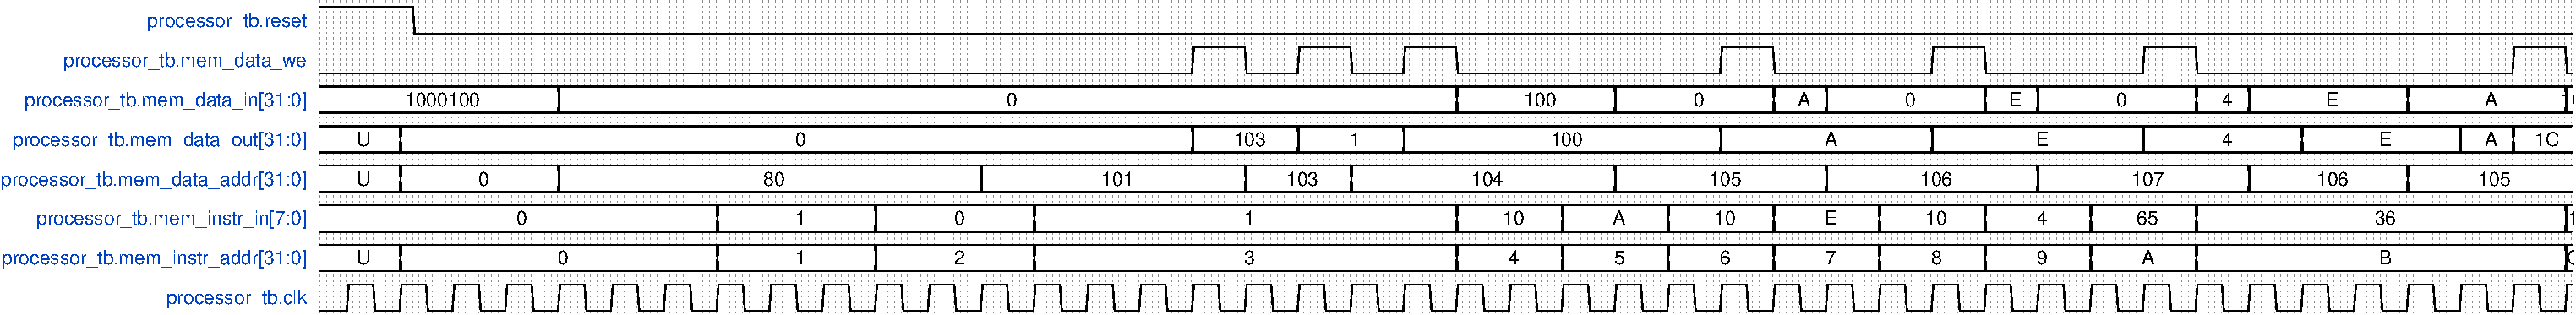
\includegraphics[width=\linewidth]{img/processor_tb.pdf}
    \caption{Simulazione del programma}
    \label{fig:processor_tb}
\end{figure}